\documentclass[JCDReport.tex]{subfiles} 
\begin{document}

The synchronization server propagates changes from one machine to another using a network connection. The management of the distributed VFSs is made on an account basis, i.e. in order to use the server, a user must have an account and link a virtual disk to this account. Therefore the server allows user to register and login after successful registration. Once the user enters the online mode (see GUI part) the currently open disk is synchronized to the server automatically. After initial synchronization, every synchronized disk gets a unique ID, so the disk can be identified. A user can have multiple disks, while a disk belongs to a single user. Unlinked disks are not synchronized. There is an automatic conflict recognition so the user can resolve conflicts by rolling back to a specific version, which is not conflicted, and then restart the synchronization again.\\

Technically the server is implemented as a WCF \footnote{http://msdn.microsoft.com/en-us/library/dd456779.aspx} service  and it allows multiple parallel connections. A an optional requirement, automatic persistence was implemented using SQLite. The usage of SQLite for this optional requirement was allowed by Alexey Kolesnichenko \footnote{https://piazza.com/class\#spring2013/252028400l/41}.\\

\subsection{Requirements}

% TODO: Remove this text and replace it with actual content
\emph{Describe which requirements (and possibly bonus requirements) you have implemented in this part. Give a quick description (1-2 sentences) of each requirement. List the software elements (classes and or functions) that are mainly involved in implementing each requirement.}


% 1. The browser should allow the user to create a new account or to log in to an existing account.
\subsubsection{Registration and login}
There are two forms for registration and login.\\
Classes: MainViewModel, DiskServiceClient\\
Commands: LoginCommand, LogoutCommand

\begin{figure}[h!]
	\centering
	\begin{subfigure}[b]{1\textwidth}
		\centering
		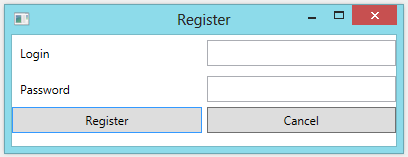
\includegraphics[scale=1]{Images/registration.png}
		\caption{Registration functionality}
	\end{subfigure}
	
	\begin{subfigure}[b]{1\textwidth}
		\centering
		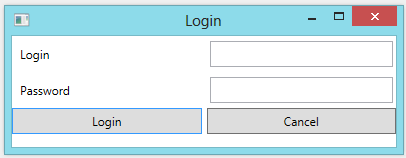
\includegraphics[scale=1]{Images/login.png} 
		\caption{Login functionality}
	\end{subfigure}
	\caption{Registration and login}
\end{figure}

% 2. The browser should offer to switch to an offine mode, and be able to operate without a connection to the server.
\subsubsection{Online / offline mode}
The user can switch between online and offline mode.\\
Classes: MainViewModel, DiskServiceClient, SynchronizationViewModel, SynchronizationService\\
Commands: SwitchToOnlineModeCommand, SwitchToOfflineModeCommand
\begin{figure}[h!]
	\centering
	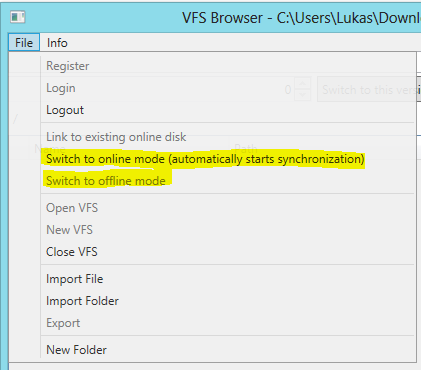
\includegraphics[scale=1]{Images/onlineofflinemode.png} 
	\caption{Online and offline switch}
\end{figure}	

% 3. The browser should support binding an existing virtual disk to an active account.
\subsubsection{Binding of existing disk}
The user can bind an existing disk to the local machine. Synchronization will then start automatically.\\
Classes: MainViewModel, DiskBrowserViewModel, DiskServiceClient\\
Commands: LinkDiskCommand
\begin{figure}[h!]
	\centering
	
\includegraphics[scale=1]{Images/todo.png} 
	\caption{Binding an existing virtual disk}
\end{figure}	

% 1. The server should support registration of unique accounts. Each account includes name & password.
\subsubsection{Registration of unique accounts}
The server provides a registration of unique user accounts. Each account includes name and password. To make registered users persistent, SQLite is used. If persistence would not have been implemented, a dictionary with the login as key could have been used.\\
Classes: UserDto, DiskServiceImpl, PersistenceImpl
\begin{figure}[h!]
	\centering
	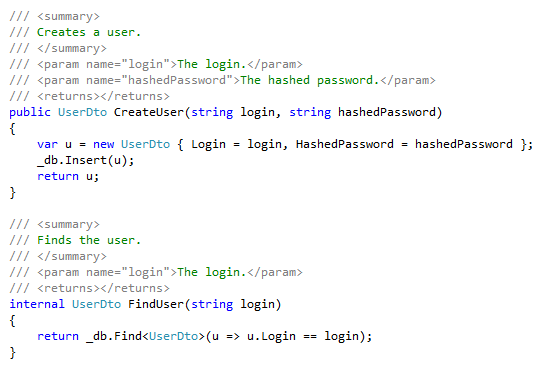
\includegraphics[scale=1]{Images/login_server.png} 
	\caption{Code to persist and to find a user}
\end{figure}

% 2. The server should track changes to linked virtual disks of registered accounts and synchronize the changes across the machines.
\subsubsection{Atuomatic synchronization across machines}
Once a disk is bound to a server and the client is in online mode, the local changes are synchronized across the machines automatically. If remote changes occur, the client automatically downloads all changes from the server.
\begin{figure}[h!]
	\centering
	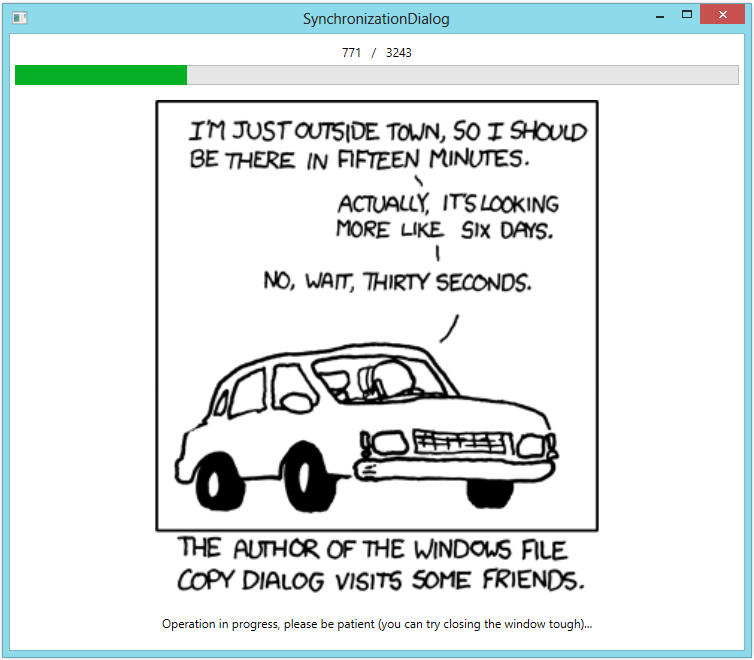
\includegraphics[scale=0.7]{Images/synchronization_dialog.png} 
	\caption{The synchronization dialogue}
\end{figure}

% 1. Provide a set of mocked unit tests for your implemenation.
\subsubsection{Mocked unit tests}
Because of the IoC pattern, mocked unit tests are fairly easy to implement. For example, in the VFSConsoleTests project, the FileSystemTextManipulatorMock mocks the FileSystemTextManipulator. Therefore the console can be tested without the FileSystemTextManipulator. Additionally, there are InOutMocks to mock the input / output.
\begin{figure}[h!]
	\centering
	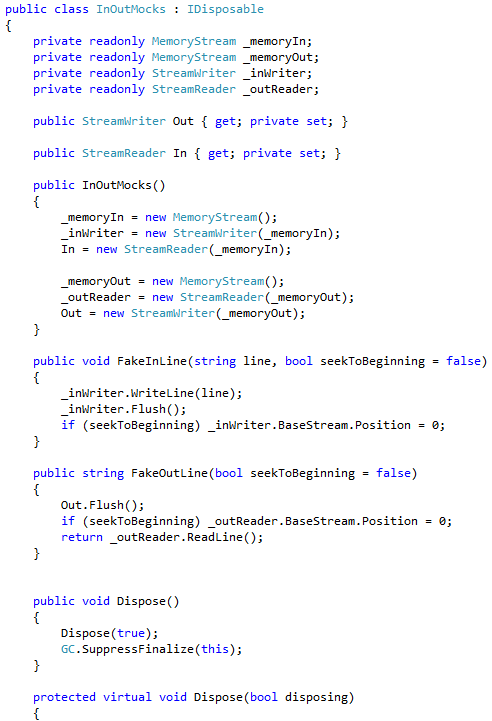
\includegraphics[scale=1]{Images/inoutmocks.png} 
	\caption{The input / output mocks to test the console application}
\end{figure}

% 2. Conflict Resolution: implement a conflict resolution scheme, so that concurrent changes to the same file are not lost (e.g. saving conflicting files as separate versions).
\subsubsection{Conflict resolution}
There is an automatic conflict recognition so the user can resolve conflicts by rolling back to a specific version, which is not conflicted, and then restart the synchronization again.\\
While the file system is conflicted, read operations are still possible. This way, the user can export a file he changed, roll back to a older version, synchronize the disk, and then import the file he changed again.

\begin{figure}[h!]
	\begin{subfigure}[b]{1\textwidth}
		\centering
		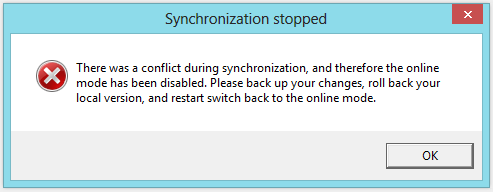
\includegraphics[scale=1]{Images/synchronization_conflict1.png}
		\caption{Conflict recognition\\\ \\} % hack for line break
	\end{subfigure}
	
	\begin{subfigure}[b]{1\textwidth}
		\centering
		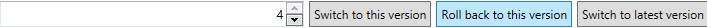
\includegraphics[scale=0.75]{Images/synchronization_conflict2.png}
		\caption{Conflict resolution}
	\end{subfigure}
	\caption{Conflict recognition and resolution}
\end{figure}


% 1. The browser is updating automatically when changes to the disk occur.
\subsubsection{Automatic updates}
The browser is updating automatically when changes to the disk occur. To make this possible, the file system provides an event, which fires when changes to the file system occur. The GUI registers to this event. This is the .NET / WPF implementation which is very similar to the observer pattern.\\
Classes: FileSystem, FileSystemTextManipulator, MainViewModel\\
Events: FileSystemChanged

\begin{figure}[h!]
	\begin{subfigure}[b]{1\textwidth}
		\centering
		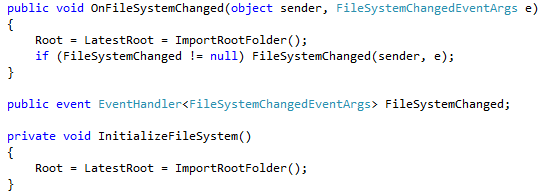
\includegraphics[scale=1]{Images/file_system_changed1.png} 
		\caption{Automatic updates: the event implementation in the file system class\\\ \\} % hack for line break
	\end{subfigure}
	
	\begin{subfigure}[b]{1\textwidth}
		\centering
		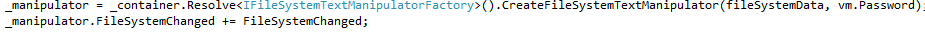
\includegraphics[scale=1]{Images/file_system_changed2.png} 
		\caption{Automatic updates: the MainViewModel registers to updates when the file system is changed\\}
	\end{subfigure}
	
	\begin{subfigure}[b]{1\textwidth}
		\centering
		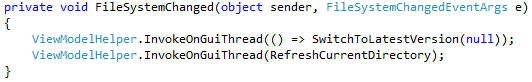
\includegraphics[scale=1]{Images/file_system_changed3.png} 
		\caption{Automatic updates: Is executed when the file system is changed\\}
	\end{subfigure}
	\caption{Automatic updates}
\end{figure}


% 2. The server is able to synchronize changes, which are done simultaneously on the same account on different machines.
\subsubsection{Simultaneous synchronization}
The server is implemented as a WCF \footnote{http://msdn.microsoft.com/en-us/library/dd456779.aspx} service  and it allows multiple parallel connections.\\
For every new connection, a new IDiskService is instantiated. This allows multiple connections to the server and thus parallel synchronization of changes. This is achieved by setting the ServiceBehavior.ConcurrencyMode to ConcurrencyMode.Multiple. To avoid additional overhead, the service is instantiated PerSession, meaning that every client creates a new service instance on the server.\\
Classes: IDiskService, DiskServiceImpl, ServiceContract

\begin{figure}[h!]
	\begin{subfigure}[b]{1\textwidth}
		\centering
		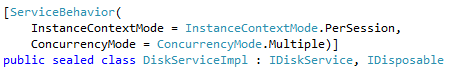
\includegraphics[scale=1]{Images/parallel_sync1.png} 
		\caption{Attributes to enable parallelism of the disk service\\\ \\\ \\} % hack for line break
	\end{subfigure}
	
	\begin{subfigure}[b]{1\textwidth}
		\centering
		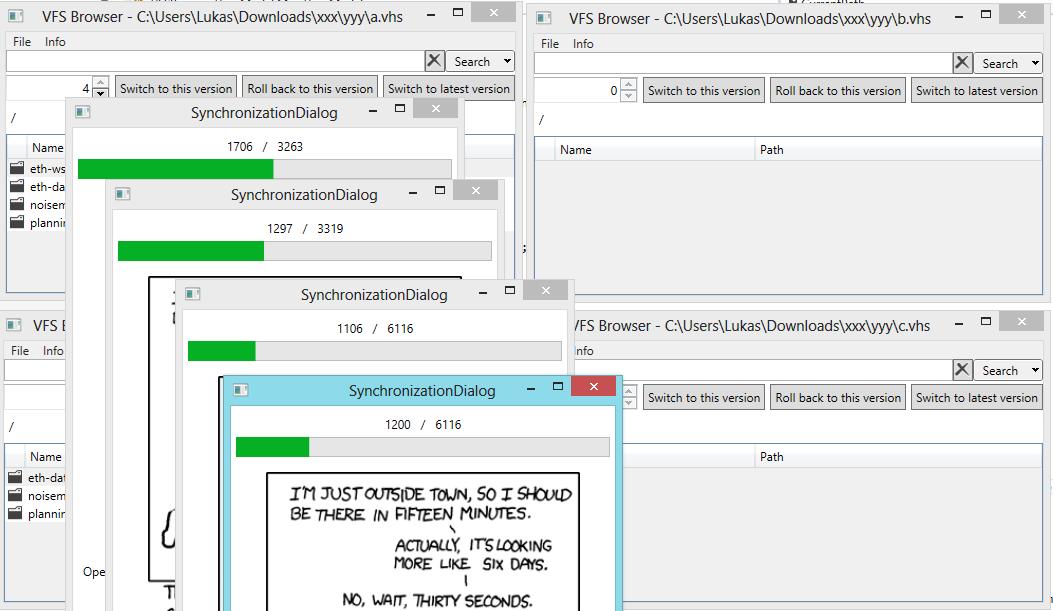
\includegraphics[scale=0.5]{Images/parallel_sync2.png} 
		\caption{Demonstration of multiple simultaneous synchronization with one running server and two different disks (three of them linked, one of them separate)}
	\end{subfigure}
	
	\caption{Simultaneous synchronization}
\end{figure}

% Incremental Changes: minimize the communication between the browser and the server by only transfering the parts of a file that changed.
\subsubsection{Incremental changes}
The synchronization only requires to synchronize the blocks which have not been synchronized before.\\
For this, the DiskDto (persisted on the server) stores the NewestBlock which is to synchronize. Locally, every file system stores the blocks used in the root folder (BlocksUsed property) of the current version. When the synchronization starts, only $$Math.abs(NewestBlock_{OnServer}-BlocksUsed_{Locally})$$ have to be synchronized.\\
Classes: SynchronizationService

\begin{figure}[h!]
	\begin{subfigure}[b]{1\textwidth}
		\centering
		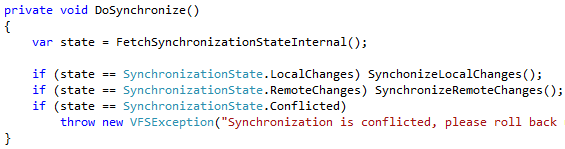
\includegraphics[scale=1]{Images/do_synchronization.png} 
		\caption{Synchronize remote changes or local changes\\\ \\} % hack for line break
	\end{subfigure}
	
	\begin{subfigure}[b]{1\textwidth}
		\centering
		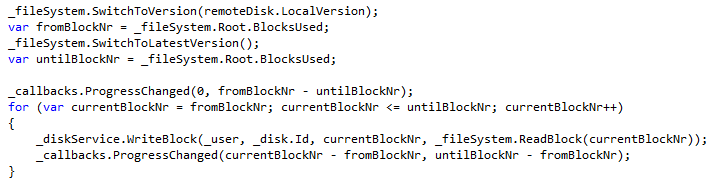
\includegraphics[scale=1]{Images/incremental_changes.png}
		\caption{Only synchronize blocks which have not been synchronized yet}
	\end{subfigure}
	\caption{Incremental changes}
\end{figure}



% 3. File History: provide a history for les and an interface to restore a previous version.
\subsubsection{File history}
There is a file history available. The user can switch to an older version and export files from there, and he also can roll back to an older version, discarding all changes in later versions.\\
Technically, the file history is implemented like this:\\
In the beginning, there is one root node. Every change in the file system then leads to a new root node, which points back to the old root node. The new root node contains block references to all children of the old root node which have not been changed during the update of the file system. Additionally, the new root node contains references to the newly created nodes. So, for every version of the history, a new root node is created. The file system options, which are stored at the start of the file system, point to the latest root node in the file system.\\



\parbox{\textwidth}{
\textbf{Example}\\
\textbf{Given:} The $root folder_{v1}$ contains a $folder a_{v1}$ and $b_{v1}$. $folder a_{v1}$ also contains a subfolder $folder x_{v1}$. The options point to the $root folder_{v1}$.\\
\textbf{Scenario:} Now a new subfolder $y_{v2}$ should be created within the folder $a_{v1}$.\\
\textbf{Action:} Then a new folder $a_{v2}$ is created, which references to the new subfolder $y_{v2}$ and to the old folder $folder a_{v1}$. Next, a new $root folder_{v2}$ is created. It creates a back link to $root folder_{v1}$, so it can switch back to an older version. Additionally, the new $root folder_{v2}$ contains a reference to the folder $b_{v1}$ (old reference) and a reference to $a_{v2}$ (new reference).\\
\textbf{Termination:} After this, the options now point to the $root folder_{v2}$.\\
\\
}

This gives us multiple advantages: Firstly, a written block never will change again (immutable object pattern). Therefore, synchronization is faster, because only the newly created blocks have to be synchronized. Furthermore, copy operations do not depend on the file size or the amount to copy. Thus the time to copy only depends on the length of the path of the files to copy.\\
Classes: FileSystem, BlockList\\
Methods: FileSystem.ArchiveAndReplaceRoot, BlockList.CopyReplacingReference

\begin{figure}[h!]
	\begin{subfigure}[b]{1\textwidth}
		\centering
		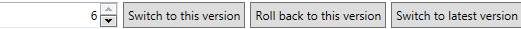
\includegraphics[scale=1]{Images/history.png}
		\caption{The file history GUI}
	\end{subfigure}
	
	\begin{subfigure}[b]{1\textwidth}
		\centering
		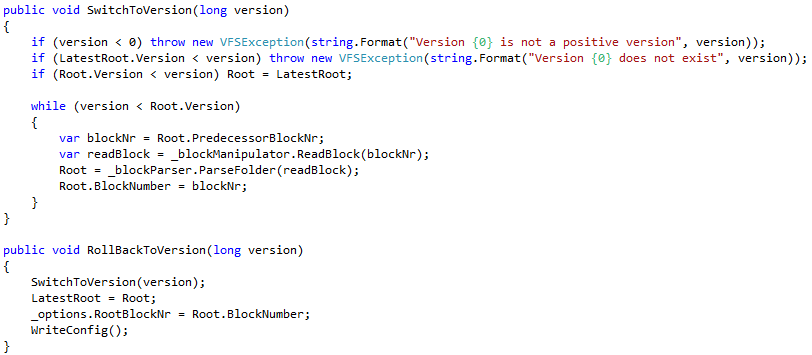
\includegraphics[scale=0.5]{Images/history_implementation.png}
		\caption{The file history implementation (FileSystem)}
	\end{subfigure}
	
	\begin{subfigure}[b]{1\textwidth}
		\centering
		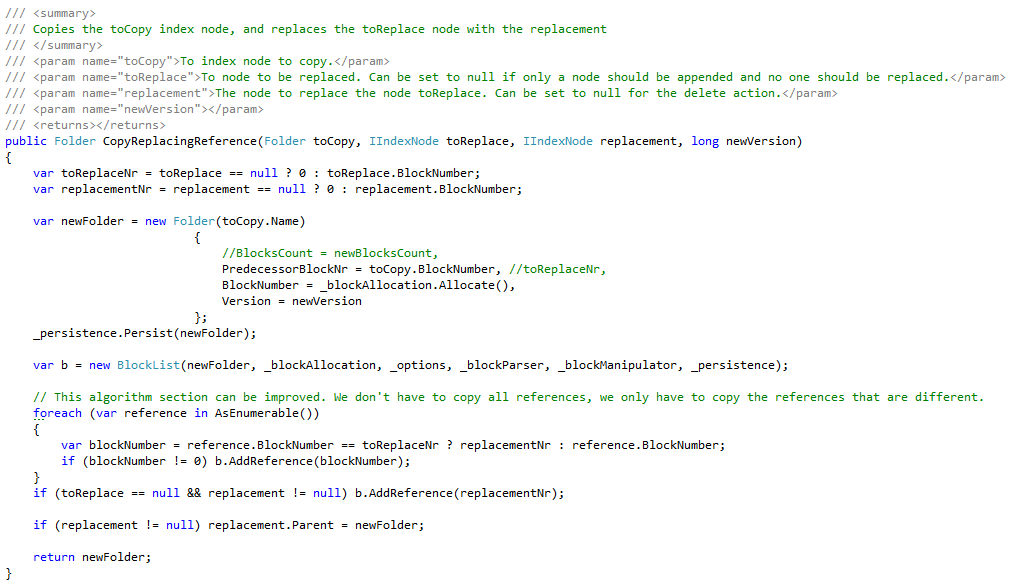
\includegraphics[scale=0.5]{Images/history_copy_replacing_reference.png}
		\caption{The file history implementation (BlockList.CopyReplacingReference)}
	\end{subfigure}
	\caption{File history}
\end{figure}


\subsection{Design}

% TODO: Remove this text and replace it with actual content
\emph{Give an overview of the design of this part and describe in general terms how the implementation works. You can mention design patterns used, class diagrams, definition of custom file formats, network protocols, or anything else that helps understand the implementation.}


\subsection{Integration}

% If you had to change the design or API of the previous part, describe the changes and the reasons for each change here.

Most of the existing design / API did not change, but it had to be enhanced for the server synchronization part. Especially, the FileSystemManipulator and the FileSystem now had to be thread safe, because the synchronization can run in the background.\\

Additionally, some existing functionality was replaced / dropped because of the history functionality and the immutable blocks. For example, the free memory command is not necessary because with the history, there is no scenario where memory is freed.\\

One very good thing were the tests. They only changed very little since they were written, and they provided immediate feedback, if something went wrong during a refactoring or by enhancing the system. The also run very fast and are run parallel by the Visual Studio 2012.

\end{document}













